\documentclass[12pt]{article}

\usepackage{graphicx}
\usepackage{amsmath}
\usepackage{amssymb}
\usepackage{natbib}
\usepackage{amsfonts}
\usepackage{multicol}
\usepackage{float}
\usepackage{oldgerm}
\usepackage{bm}
\usepackage{mathtools}
\usepackage{wrapfig}
\usepackage{fancyhdr}
\usepackage[export]{adjustbox}
\usepackage{xcolor}

\pagestyle{empty}

\newcommand{\Avec}{\mathbf A}
\newcommand{\Bvec}{\mathbf B}
\newcommand{\Dvec}{\mathbf D}
\newcommand{\Evec}{\mathbf E}
\newcommand{\Fvec}{\mathbf F}
\newcommand{\Jvec}{\mathbf J}
\newcommand{\Lvec}{\mathbf L}
\newcommand{\Mvec}{\mathbf M}
\newcommand{\Pvec}{\mathbf P}
\newcommand{\Svec}{\mathbf S}
\newcommand{\avec}{\mathbf a}
\newcommand{\bvec}{\mathbf b}
\newcommand{\dvec}{\mathbf d}
\newcommand{\evec}{\mathbf e}
\newcommand{\fvec}{\mathbf f}
\newcommand{\jvec}{\mathbf j}
\newcommand{\kvec}{\mathbf k}
\newcommand{\nvec}{\mathbf n}
\newcommand{\pvec}{\mathbf p}
\newcommand{\rvec}{\mathbf r}
\newcommand{\svec}{\mathbf s}
\newcommand{\vvec}{\mathbf v}
\newcommand{\xvec}{\mathbf x}
\newcommand{\yvec}{\mathbf y}
\newcommand{\zvec}{\mathbf z}
\newcommand{\nablav}{\boldsymbol{\nabla}}
\newcommand{\nablavector}{\vec \nabla}
\newcommand{\alphavec}{\boldsymbol{\alpha}}
\newcommand{\phivec}{\boldsymbol{\phi}}
\newcommand{\thetavec}{\boldsymbol{\theta}}
\newcommand{\omegavec}{\boldsymbol{\omega}}
\newcommand{\tauvec}{\boldsymbol{\tau}}
\newcommand{\ezero}{\varepsilon_{0}}
\newcommand{\mzero}{\mu_{0}}
\newcommand{\mubold}{\boldsymbol{\mu}}
\newcommand{\uniti}{\hat{\boldsymbol{\imath}}}
\newcommand{\unitj}{\hat{\boldsymbol{\jmath}}}
\newcommand{\unitk}{\hat{\boldsymbol{\mathit{k}}}}
\newcommand{\unitn}{\hat{\mathbf n}}
\newcommand{\unitr}{\hat{\mathbf r}}
\newcommand{\unitphi}{\hat{\boldsymbol{\phi}}}
\newcommand{\unittheta}{\hat{\boldsymbol{\theta}}}

\newcommand{\bit}{\begin{itemize}}
\newcommand{\eit}{\end{itemize}}

\setlength{\headsep}{0.5cm}
\setlength{\oddsidemargin}{-0.5cm}
\setlength{\textwidth}{16.5cm}
\setlength{\textheight}{24cm}
\voffset = -2cm

\pagestyle{fancy}
\fancyhf{}
\rfoot{
\includegraphics[width=1.0in]{cnm.png}}
\lfoot{ENGR 2910 Homework 6}

\begin{document}

%{\bf \underline{STUDENT NAME}:} 
%\vspace{1cm}

\begin{center}
%\date{10/02/18-10/09/18}
\hfil
{\large\bf {ENGR 2910-101: Circuit Analysis}}
\hfill Instructor: Leo Silbert \\
Homework 6: 10/06/21 \hfill Due: 10/13/21\\
\hrulefill\\
\end{center}

%{\em Show all your working to ensure you obtain full points. Partial
%  credit will be given for correct algebraic steps if you fail to
%  obtain the correct final answer.}\\

%\newpage


\noindent
{\bf Question 1} [10]

For the current-divider circuit shown here calculate:
\begin{figure}[h!]
  \centering 
 \vspace{-0.1in}
 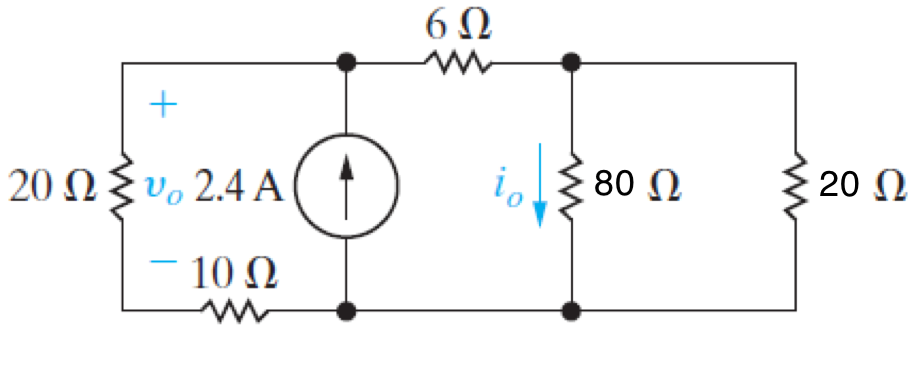
\includegraphics[clip,width=0.8\textwidth]{Fig3-19.png}
 %\vspace{-0.1in}
\end{figure}

\bit

\item[(i)]

$i_{o}$ and $v_{o}$,

\item[(ii)]

the power dissipated in the 6 $\Omega$ resistor,

\item[(iii)]

the power delivered by the current source.

\eit

\vspace{0.1in}
\noindent
{\bf Question 2} [10]

For the circuit shown, calculate $i_{1}$ and $i_{2}$ using current-division.
\begin{figure}[h!]
     \centering
\vspace{-0.1in}
     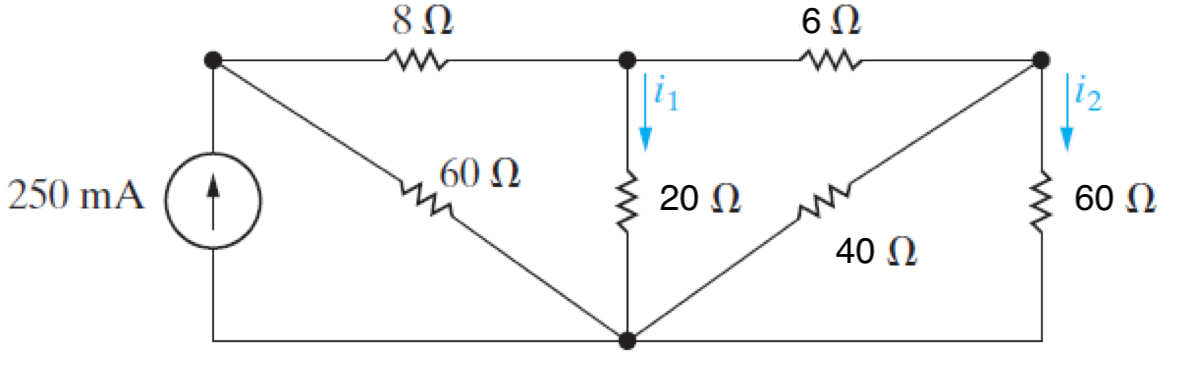
\includegraphics[clip,width=0.9\textwidth]{Fig3-29.png}
\vspace{-0.15in}
\end{figure}
 \newpage
\noindent
{\bf Question 3} [10]

Use a $\Delta$-to-$Y$ transformation to find the voltages $v_{1}$ and
$v_{2}$ in the circuit below. 

\begin{figure}[!h]
  \centering 
  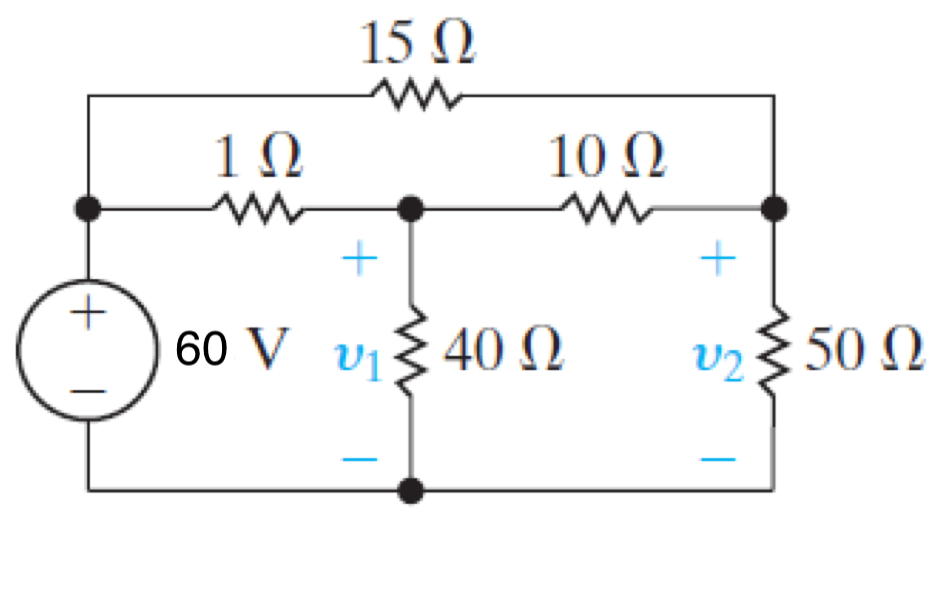
\includegraphics[clip,width=0.4\textwidth]{Fig3-58.png}
\end{figure}

\vspace{0.1in}
\noindent
{\bf Question 4} [10]

Use a $Y$-to-$\Delta$ transformation to find the equivalent resistance
$R_{ab}$. 
\begin{figure}[h!]
  \centering 
  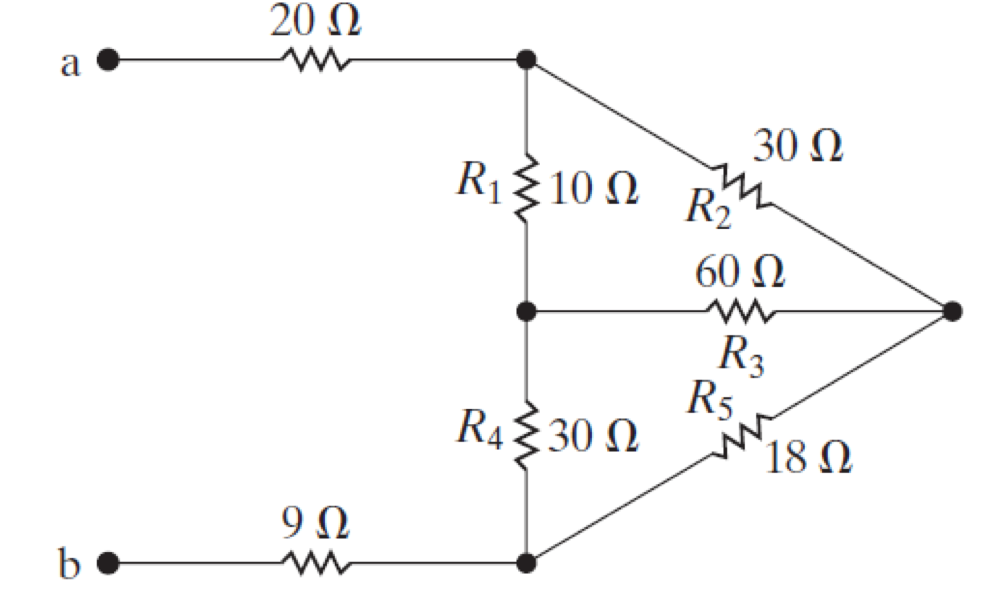
\includegraphics[clip,width=0.6\textwidth]{Fig3-61.png}
\end{figure}

\vspace{0.1in}
\noindent
{\bf Question 5} [10]

For the circuit circuit shown:
\begin{figure}[h!]
\centering 
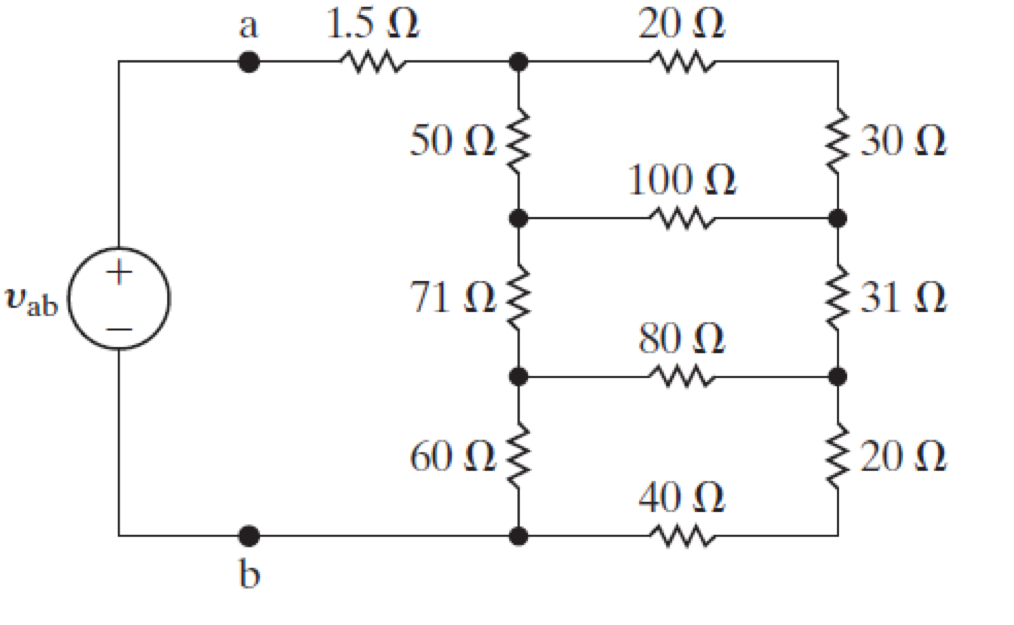
\includegraphics[clip,width=0.6\textwidth]{Fig3-63.png}
\end{figure}
 \bit

\item[(a)]

Find the resistance seen by the ideal voltage source. 

\item[(b)]

If $v_{ab} = 250$ V, how much power is dissipated in the 31 $\Omega$ resistor?

\eit

\end{document}
